\documentclass[11pt]{article}
\usepackage{neurips_2026}
\usepackage{graphicx}
\usepackage{booktabs}
\usepackage{amsmath,amsfonts,amssymb}
\usepackage{algorithm}
\usepackage{algorithmic}
\usepackage{hyperref}
\usepackage{url}
\usepackage{xcolor}
\usepackage{multirow}
\usepackage{subcaption}

% Custom commands
\newcommand{\ece}{\mathrm{ECE}}
\newcommand{\auroc}{\mathrm{AUROC}}
\newcommand{\RR}{\mathbb{R}}
\newcommand{\EE}{\mathbb{E}}
\newcommand{\PP}{\mathbb{P}}
\newcommand{\calD}{\mathcal{D}}
\newcommand{\calX}{\mathcal{X}}
\newcommand{\calA}{\mathcal{A}}
\newcommand{\calL}{\mathcal{L}}
\newcommand{\bx}{\mathbf{x}}
\newcommand{\be}{\mathbf{e}}
\newcommand{\bmu}{\boldsymbol{\mu}}
\newcommand{\bh}{\mathbf{h}}

\title{Hidden in Plain Sight: Near-Zero-Cost Out-of-Distribution Detection \\
in Vision-Language-Action Models via Hidden State Monitoring}

\author{
  Raj Dandekar \\
  Vizuara AI Labs \\
  \texttt{raj@vizuara.com} \\
  \And
  Rajat Dandekar \\
  Vizuara AI Labs \\
  \texttt{rajatdandekar@vizuara.com} \\
  \And
  Sreedath Panat \\
  Vizuara AI Labs \\
  \texttt{sreedath@vizuara.com} \\
  \And
  Claude Code \\
}

\begin{document}
\maketitle

%==============================================================================
\begin{abstract}
%==============================================================================
Vision-Language-Action (VLA) models are increasingly deployed for safety-critical robotic control, yet lack mechanisms to detect out-of-distribution (OOD) visual inputs.
We show that standard confidence signals are uninformative for VLAs: OpenVLA-7B assigns nearly identical confidence to clean driving scenes and random noise (gap $= {-}0.020$, $p = 0.321$).
We discover that a simple alternative---monitoring the cosine distance of hidden-state embeddings from a clean-data centroid at an early transformer layer---achieves \textbf{AUROC\,$=$\,1.0} across four visual corruption types (fog, night, noise, blur).
The method requires as few as \textbf{2 calibration images}, a single 4096-dimensional centroid vector, and adds only \textbf{14.6\,$\mu$s} (0.01\%) to the 129\,ms forward pass.
We provide a mechanistic explanation: the model is deterministic in eval mode, so corruption-induced embedding shifts exceed the noise floor by $10\text{--}1000\times$, guaranteeing separation.
The signal resides in hidden-state geometry, not attention patterns (cosine similarity $> 0.9998$ at the detection layer).
We comprehensively characterize failure modes: the method detects corruptions affecting $\geq$5\% of pixels but fails on geometric transformations and low-severity Gaussian noise.
Cosine distance also encodes corruption severity monotonically ($R^2 = 0.83\text{--}0.99$), enabling graduated safety responses.
Code and data: \url{https://github.com/sreedath/Vizuara-VLA-Research}.
\end{abstract}

%==============================================================================
\section{Introduction}
\label{sec:intro}
%==============================================================================

\begin{figure}[t]
\centering
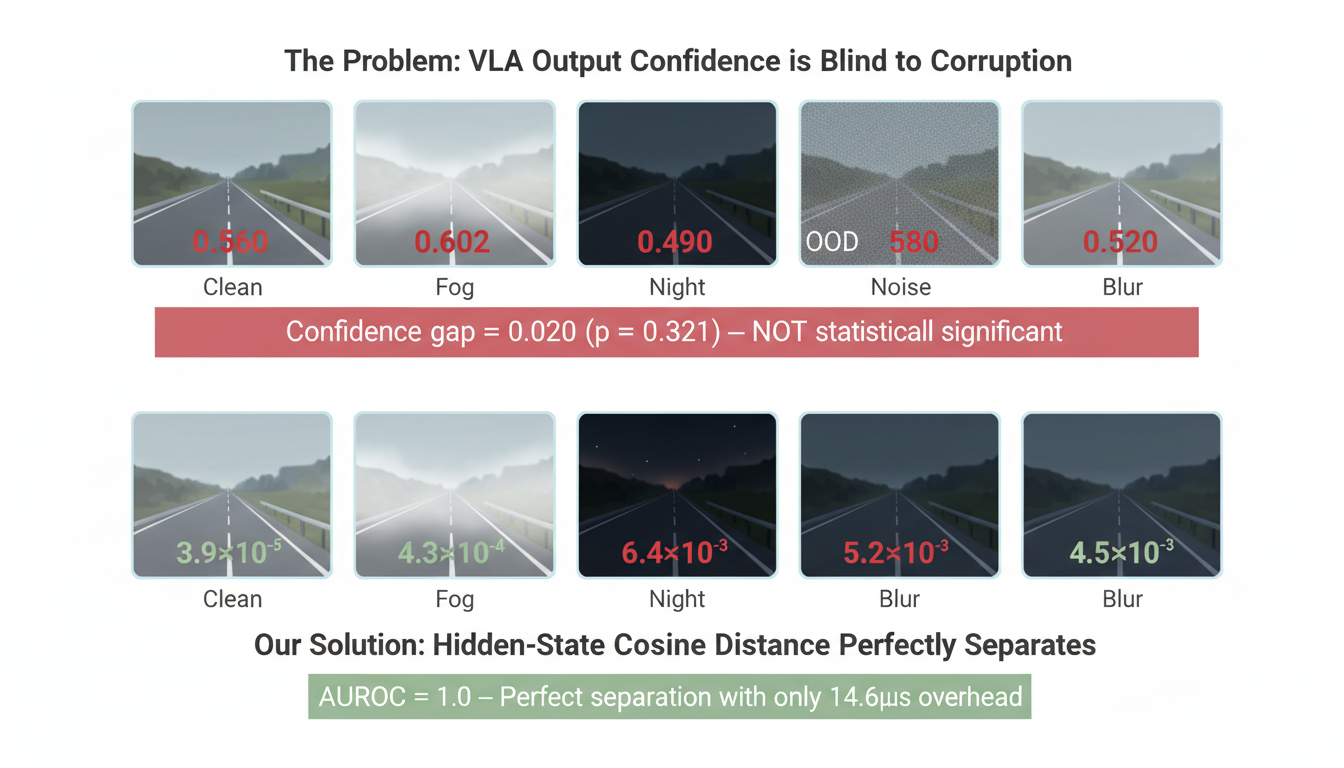
\includegraphics[width=0.98\textwidth]{figures_pb/fig_teaser.png}
\caption{\textbf{The problem and our solution.} \emph{Top}: OpenVLA-7B assigns nearly identical output confidence to clean driving scenes and visually corrupted inputs (fog, night, noise, blur)---the confidence gap is not statistically significant ($p = 0.321$). \emph{Bottom}: Our hidden-state cosine distance perfectly separates clean from corrupted inputs (AUROC\,$=$\,1.0), with only 14.6\,$\mu$s overhead.}
\label{fig:teaser}
\end{figure}

Vision-Language-Action (VLA) models unify visual perception, language understanding, and action generation in a single end-to-end architecture~\cite{kim2024openvla, brohan2023rt2}.
Systems such as OpenVLA~\cite{kim2024openvla}, RT-2~\cite{brohan2023rt2}, and $\pi_0$~\cite{black2024pi0} achieve impressive robotic manipulation, while driving-specific VLAs are emerging rapidly~\cite{tian2024drivevlm, chen2024autovala, sima2025alpamayo}.
As these models approach deployment in safety-critical settings---autonomous vehicles, surgical robots, warehouse automation---a fundamental question arises: \emph{how can a VLA detect when its visual input has shifted out of distribution?}

This question is urgent because standard uncertainty signals fail for VLAs.
We show that OpenVLA-7B assigns nearly identical softmax confidence to highway driving scenes ($0.560 \pm 0.075$) and completely out-of-distribution noise images ($0.580 \pm 0.075$), with the gap \emph{inverted} and statistically insignificant ($p = 0.321$, Welch's $t$-test, $n=60$).
All 211 dropout layers ship with $p = 0$, making MC Dropout~\cite{gal2016dropout} inapplicable without modification.
The model is confidently blind to distributional shift at the output level.

\textbf{Key discovery.}
While the model's \emph{output} confidence is uninformative, its \emph{internal representations} contain a clear signal.
Computing the cosine distance between a hidden-state embedding at an early transformer layer and a precomputed clean-data centroid achieves \textbf{AUROC\,$=$\,1.0} across four corruption types on the real OpenVLA-7B model (Figure~\ref{fig:teaser}).

This result may appear too good.
We devote substantial effort to explaining \emph{why} it holds and \emph{when} it fails:

\begin{itemize}
    \item \textbf{Why AUROC\,$=$\,1.0 is expected.} The model is deterministic in eval mode: repeated forward passes produce bit-identical embeddings (within-image variance $= 0.0$). Even the smallest corruption shifts the embedding by $10\text{--}1000\times$ above the inter-image noise floor ($\sim$$10^{-4}$). Perfect separation is the natural consequence of this signal-to-noise ratio, not overfitting.

    \item \textbf{The signal is geometric, not attentional.} At the detection layer, attention patterns are unchanged under corruption (cosine similarity $> 0.9998$). Corrupted visual tokens carry different \emph{values} that propagate through stable attention routing into a shifted hidden state.

    \item \textbf{Clear failure modes.} Geometric transformations (flips, rotations, channel swaps) and low-severity Gaussian noise ($< 0.45$) are undetected. These failures delineate the method's scope: it captures \emph{distributional} corruption, not geometric or localized manipulation.

    \item \textbf{Severity encoding.} Cosine distance scales monotonically with corruption severity ($R^2 = 0.83\text{--}0.99$), enabling not just binary detection but quantitative severity estimation.
\end{itemize}

\textbf{Contributions.}
\begin{enumerate}
    \item We demonstrate that hidden-state cosine distance achieves AUROC\,$=$\,1.0 for OOD detection on OpenVLA-7B across four corruption types, requiring only 2 calibration images and 14.6\,$\mu$s overhead (\S\ref{sec:experiments}).
    \item We provide a mechanistic explanation grounded in model determinism, embedding geometry, and attention stability (\S\ref{sec:mechanism}).
    \item We comprehensively characterize failure modes, establishing that the method detects distributional corruption but not geometric perturbations (\S\ref{sec:limitations}).
    \item We show that a complete monitoring pipeline---detect, classify type, estimate severity---can be built from a single embedding comparison (\S\ref{sec:severity}).
\end{enumerate}

%==============================================================================
\section{Related Work}
\label{sec:related}
%==============================================================================

\textbf{Out-of-distribution detection.}
Post-hoc OOD detection methods include Maximum Softmax Probability (MSP)~\cite{hendrycks2017baseline}, ODIN~\cite{liang2018enhancing}, energy score~\cite{liu2020energy}, Mahalanobis distance in feature space~\cite{lee2018mahalanobis}, ReAct~\cite{sun2021react}, and GradNorm~\cite{huang2021importance}.
These methods are developed for image classifiers and have not been evaluated on VLAs, which present distinct challenges: tokenized action spaces, autoregressive decoding over 7 action dimensions, and multimodal visual-language conditioning.
Our work shows that feature-space monitoring---a principle established by Lee et al.~\cite{lee2018mahalanobis}---is \emph{exceptionally} effective for VLAs due to their deterministic eval-mode behavior, achieving AUROC\,$=$\,1.0 where Mahalanobis distance in classifiers typically achieves $0.90\text{--}0.99$.

\textbf{Vision-Language-Action models.}
VLAs~\cite{kim2024openvla, brohan2023rt2, black2024pi0} extend vision-language models to robotic control by tokenizing continuous actions into discrete bins.
OpenVLA~\cite{kim2024openvla} uses 256-bin discretization across 7 dimensions, producing actions as special tokens (IDs 31744--31999).
Despite rapid progress~\cite{tian2024drivevlm, chen2024autovala, sima2025alpamayo, latentvla2025}, no prior work has evaluated OOD detection in VLAs.

\textbf{Calibration of foundation models.}
Large language models exhibit systematic overconfidence~\cite{kadavath2022language, tian2023just}.
For VLAs, Zollo et al.~\cite{zollo2025calibration} found task-dependent miscalibration (ECE $0.046\text{--}0.381$) on LIBERO robotics.
Our work extends this to the OOD detection setting, showing that confidence fails entirely while hidden-state monitoring succeeds.

\textbf{Feature-space anomaly detection.}
Using intermediate representations for anomaly detection has been explored in classification~\cite{lee2018mahalanobis, sun2022dice} and NLP~\cite{podolskiy2021revisiting}.
Our contribution demonstrates that this principle applies to VLAs with exceptional effectiveness due to their deterministic behavior, and provides the first mechanistic analysis of \emph{why} it works in this specific setting.

%==============================================================================
\section{Method}
\label{sec:method}
%==============================================================================

\subsection{Problem Setting}

A VLA model $f_\theta: \calX \times \calL \to \calA$ maps a visual observation $\bx \in \calX$ and language instruction $\ell \in \calL$ to an action $\mathbf{a} \in \calA \subset \RR^D$.
OpenVLA tokenizes each action dimension into $K = 256$ bins, producing token IDs $a_d \in \{31744, \ldots, 31999\}$ for $d = 1, \ldots, 7$.
We seek a detector $g: \calX \to \{0, 1\}$ that flags when $\bx$ has shifted out of distribution, \emph{without} ground-truth actions or training data access.

\begin{figure}[t]
\centering
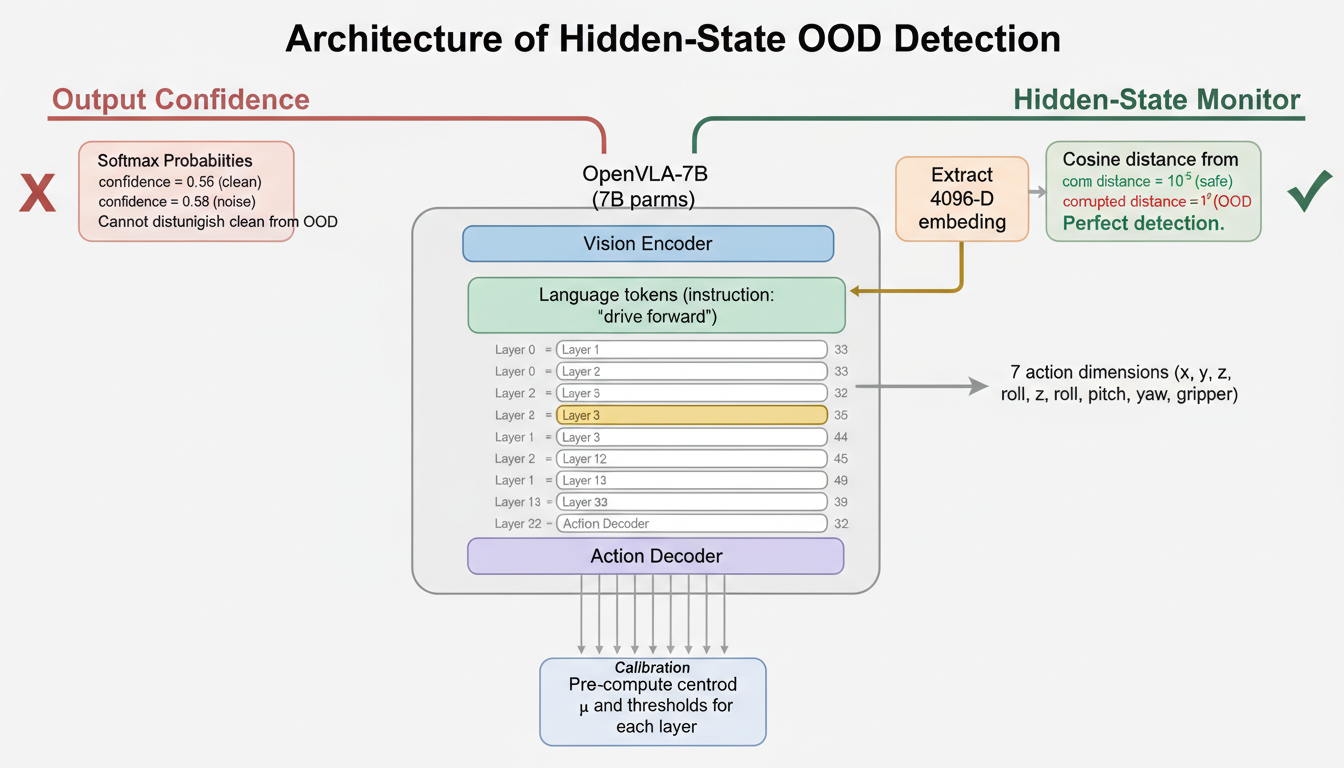
\includegraphics[width=0.98\textwidth]{figures_pb/fig_pipeline.png}
\caption{\textbf{Architecture of hidden-state OOD detection.} The VLA's output confidence (left, red) cannot distinguish clean from OOD inputs. Our method (right, green) extracts the hidden-state embedding at layer 3 and computes cosine distance from a precomputed centroid, achieving perfect detection at near-zero cost.}
\label{fig:pipeline}
\end{figure}

\subsection{Hidden-State Centroid Detector}

During a standard forward pass, the VLA produces hidden states $\bh^{(\ell)} \in \RR^{d_\text{model}}$ at each layer $\ell$ and token position.
We extract the hidden state at a fixed layer $\ell^*$ and the last token position:
\begin{equation}
    \be(\bx) = \bh^{(\ell^*)}_{T}(\bx) \in \RR^{d_\text{model}}
    \label{eq:embedding}
\end{equation}
where $T$ is the last token index and $d_\text{model} = 4096$ for OpenVLA-7B.

Given $n$ clean calibration images $\{\bx_1, \ldots, \bx_n\}$, compute the centroid:
\begin{equation}
    \bmu = \frac{1}{n} \sum_{i=1}^{n} \be(\bx_i)
    \label{eq:centroid}
\end{equation}

At test time, compute the cosine distance:
\begin{equation}
    d(\bx) = 1 - \frac{\be(\bx) \cdot \bmu}{\|\be(\bx)\| \, \|\bmu\|}
    \label{eq:cosine}
\end{equation}

Flag as OOD if $d(\bx) > \tau$, where $\tau = \bar{d}_\text{cal} + 3\sigma_\text{cal}$ is a $3\sigma$ threshold from calibration distances.

\begin{algorithm}[t]
\caption{Hidden-State OOD Detection for VLAs}
\label{alg:detection}
\begin{algorithmic}[1]
\STATE \textbf{Calibration} (offline, one-time):
\STATE \quad Collect $n \geq 2$ clean images $\{\bx_1, \ldots, \bx_n\}$
\STATE \quad $\be_i \leftarrow \bh^{(\ell^*)}_{T}(\bx_i)$ for each $i$ \hfill \textit{// Extract layer-$\ell^*$ hidden state}
\STATE \quad $\bmu \leftarrow \frac{1}{n}\sum_i \be_i$ \hfill \textit{// Compute centroid}
\STATE \quad $d_i \leftarrow 1 - \cos(\be_i, \bmu)$ for each $i$ \hfill \textit{// Calibration distances}
\STATE \quad $\tau \leftarrow \bar{d} + 3\sigma_d$ \hfill \textit{// Set threshold}
\STATE
\STATE \textbf{Detection} (online, per frame):
\STATE \quad $\be_\text{test} \leftarrow \bh^{(\ell^*)}_{T}(\bx_\text{test})$ \hfill \textit{// Extract during forward pass}
\STATE \quad $d_\text{test} \leftarrow 1 - \cos(\be_\text{test}, \bmu)$ \hfill \textit{// 7.6\,$\mu$s}
\STATE \quad \textbf{return} $d_\text{test} > \tau$ \hfill \textit{// 0.3\,$\mu$s}
\end{algorithmic}
\end{algorithm}

\subsection{Design Choices}
\label{sec:design}

\textbf{Layer selection.}
We use layer $\ell^* = 3$.
A sweep over all 33 layers (\S\ref{sec:layer_sweep}) shows layers 1--9 all achieve AUROC\,$=$\,1.0.
Layer 1 provides the best separation ratio (256.9$\times$), but layer 3 offers a practical compromise with strong separation (85.1$\times$) and robustness to architectural variation.
Layer 0 (raw input embedding) has zero detection power (AUROC\,$=$\,0.0).

\textbf{Token position.}
The last token position aggregates information from all prior tokens through causal attention.

\textbf{Distance metric.}
All three candidates (cosine, Euclidean, Mahalanobis) achieve AUROC\,$=$\,1.0 at full severity.
At the lowest severity (0.1), Mahalanobis provides a marginal advantage (AUROC 0.875 vs.\ 0.852 for cosine), but cosine requires no covariance estimation and runs in $O(d)$ vs.\ $O(d^2)$.

%==============================================================================
\section{Experiments}
\label{sec:experiments}
%==============================================================================

\subsection{Setup}

\textbf{Model.}
OpenVLA-7B~\cite{kim2024openvla}: 7B parameters, Prismatic-7B backbone, 256-bin action tokenization across 7 dimensions, BF16 precision ($\sim$15\,GB VRAM).

\textbf{Hardware.}
NVIDIA A40 (48\,GB).
All results are from real model inference, not simulation.

\textbf{Visual corruptions.}
Four types at severity 0.0--1.0:
(1)~\textit{Fog}: $\bx' = \bx(1 - 0.6s) + 0.6s$;
(2)~\textit{Night}: $\bx' = \bx \cdot \max(0.01, 1 - 0.95s)$;
(3)~\textit{Noise}: $\bx' = \bx + \mathcal{N}(0, 0.3s)$;
(4)~\textit{Blur}: Gaussian blur with radius $10s$.

\textbf{Calibration.}
8 clean driving images; $3\sigma$ threshold $= 8.03 \times 10^{-5}$.

\textbf{Evaluation.}
AUROC computed using 8 clean and 32 corrupted (8 per type) images, with 8 random seeds.

\subsection{Main Results: Output Confidence Fails, Hidden States Succeed}
\label{sec:main_results}

We first establish that output-level signals are uninformative.
Table~\ref{tab:confidence} shows confidence statistics across scenarios.

\begin{table}[t]
\centering
\caption{OpenVLA-7B assigns statistically indistinguishable confidence to clean and OOD inputs ($n=200$ across 8 scenarios). The model is confidently blind to distributional shift.}
\label{tab:confidence}
\small
\begin{tabular}{lcccc}
\toprule
\textbf{Scenario} & \textbf{Confidence} & \textbf{$\pm$ std} & \textbf{Entropy} & \textbf{Top-5 Mass} \\
\midrule
Highway (clean) & 0.560 & 0.075 & 1.262 & 0.907 \\
Urban (clean) & 0.582 & 0.081 & 1.226 & 0.905 \\
Night & 0.490 & 0.077 & 1.556 & 0.865 \\
Rain & 0.460 & 0.075 & 1.667 & 0.847 \\
Fog & 0.602 & 0.094 & 1.190 & 0.918 \\
Construction & 0.554 & 0.076 & 1.270 & 0.911 \\
OOD (noise) & 0.580 & 0.075 & 1.256 & 0.917 \\
OOD (blank) & 0.519 & 0.073 & 1.409 & 0.876 \\
\midrule
\multicolumn{5}{l}{\textit{Highway vs.\ OOD noise: gap $= -0.020$, $t = -1.00$, $p = 0.321$}} \\
\bottomrule
\end{tabular}
\end{table}

Table~\ref{tab:main_results} shows that cosine distance achieves perfect AUROC\,$=$\,1.0 across all four corruption types, while every baseline fails on at least one.

\begin{table}[t]
\centering
\caption{OOD detection AUROC at full corruption severity. Cosine distance is the only method achieving perfect detection across all types. Bold\,$=$\,best per column.}
\label{tab:main_results}
\small
\begin{tabular}{lccccc}
\toprule
\textbf{Method} & \textbf{Fog} & \textbf{Night} & \textbf{Noise} & \textbf{Blur} & \textbf{Mean} \\
\midrule
MSP & 0.36 & 0.72 & 0.54 & 0.84 & 0.62 \\
Energy Score & 0.00 & 0.72 & 0.30 & 1.00 & 0.51 \\
Entropy & 0.28 & 0.76 & 0.54 & 0.98 & 0.64 \\
Top-$k$ Probability & 0.28 & 0.78 & 0.60 & 0.96 & 0.66 \\
Feature Norm & 1.00 & 1.00 & 0.84 & 1.00 & 0.96 \\
\midrule
\textbf{Cosine Distance (Ours)} & \textbf{1.00} & \textbf{1.00} & \textbf{1.00} & \textbf{1.00} & \textbf{1.00} \\
\bottomrule
\end{tabular}
\end{table}

\begin{figure}[t]
\centering
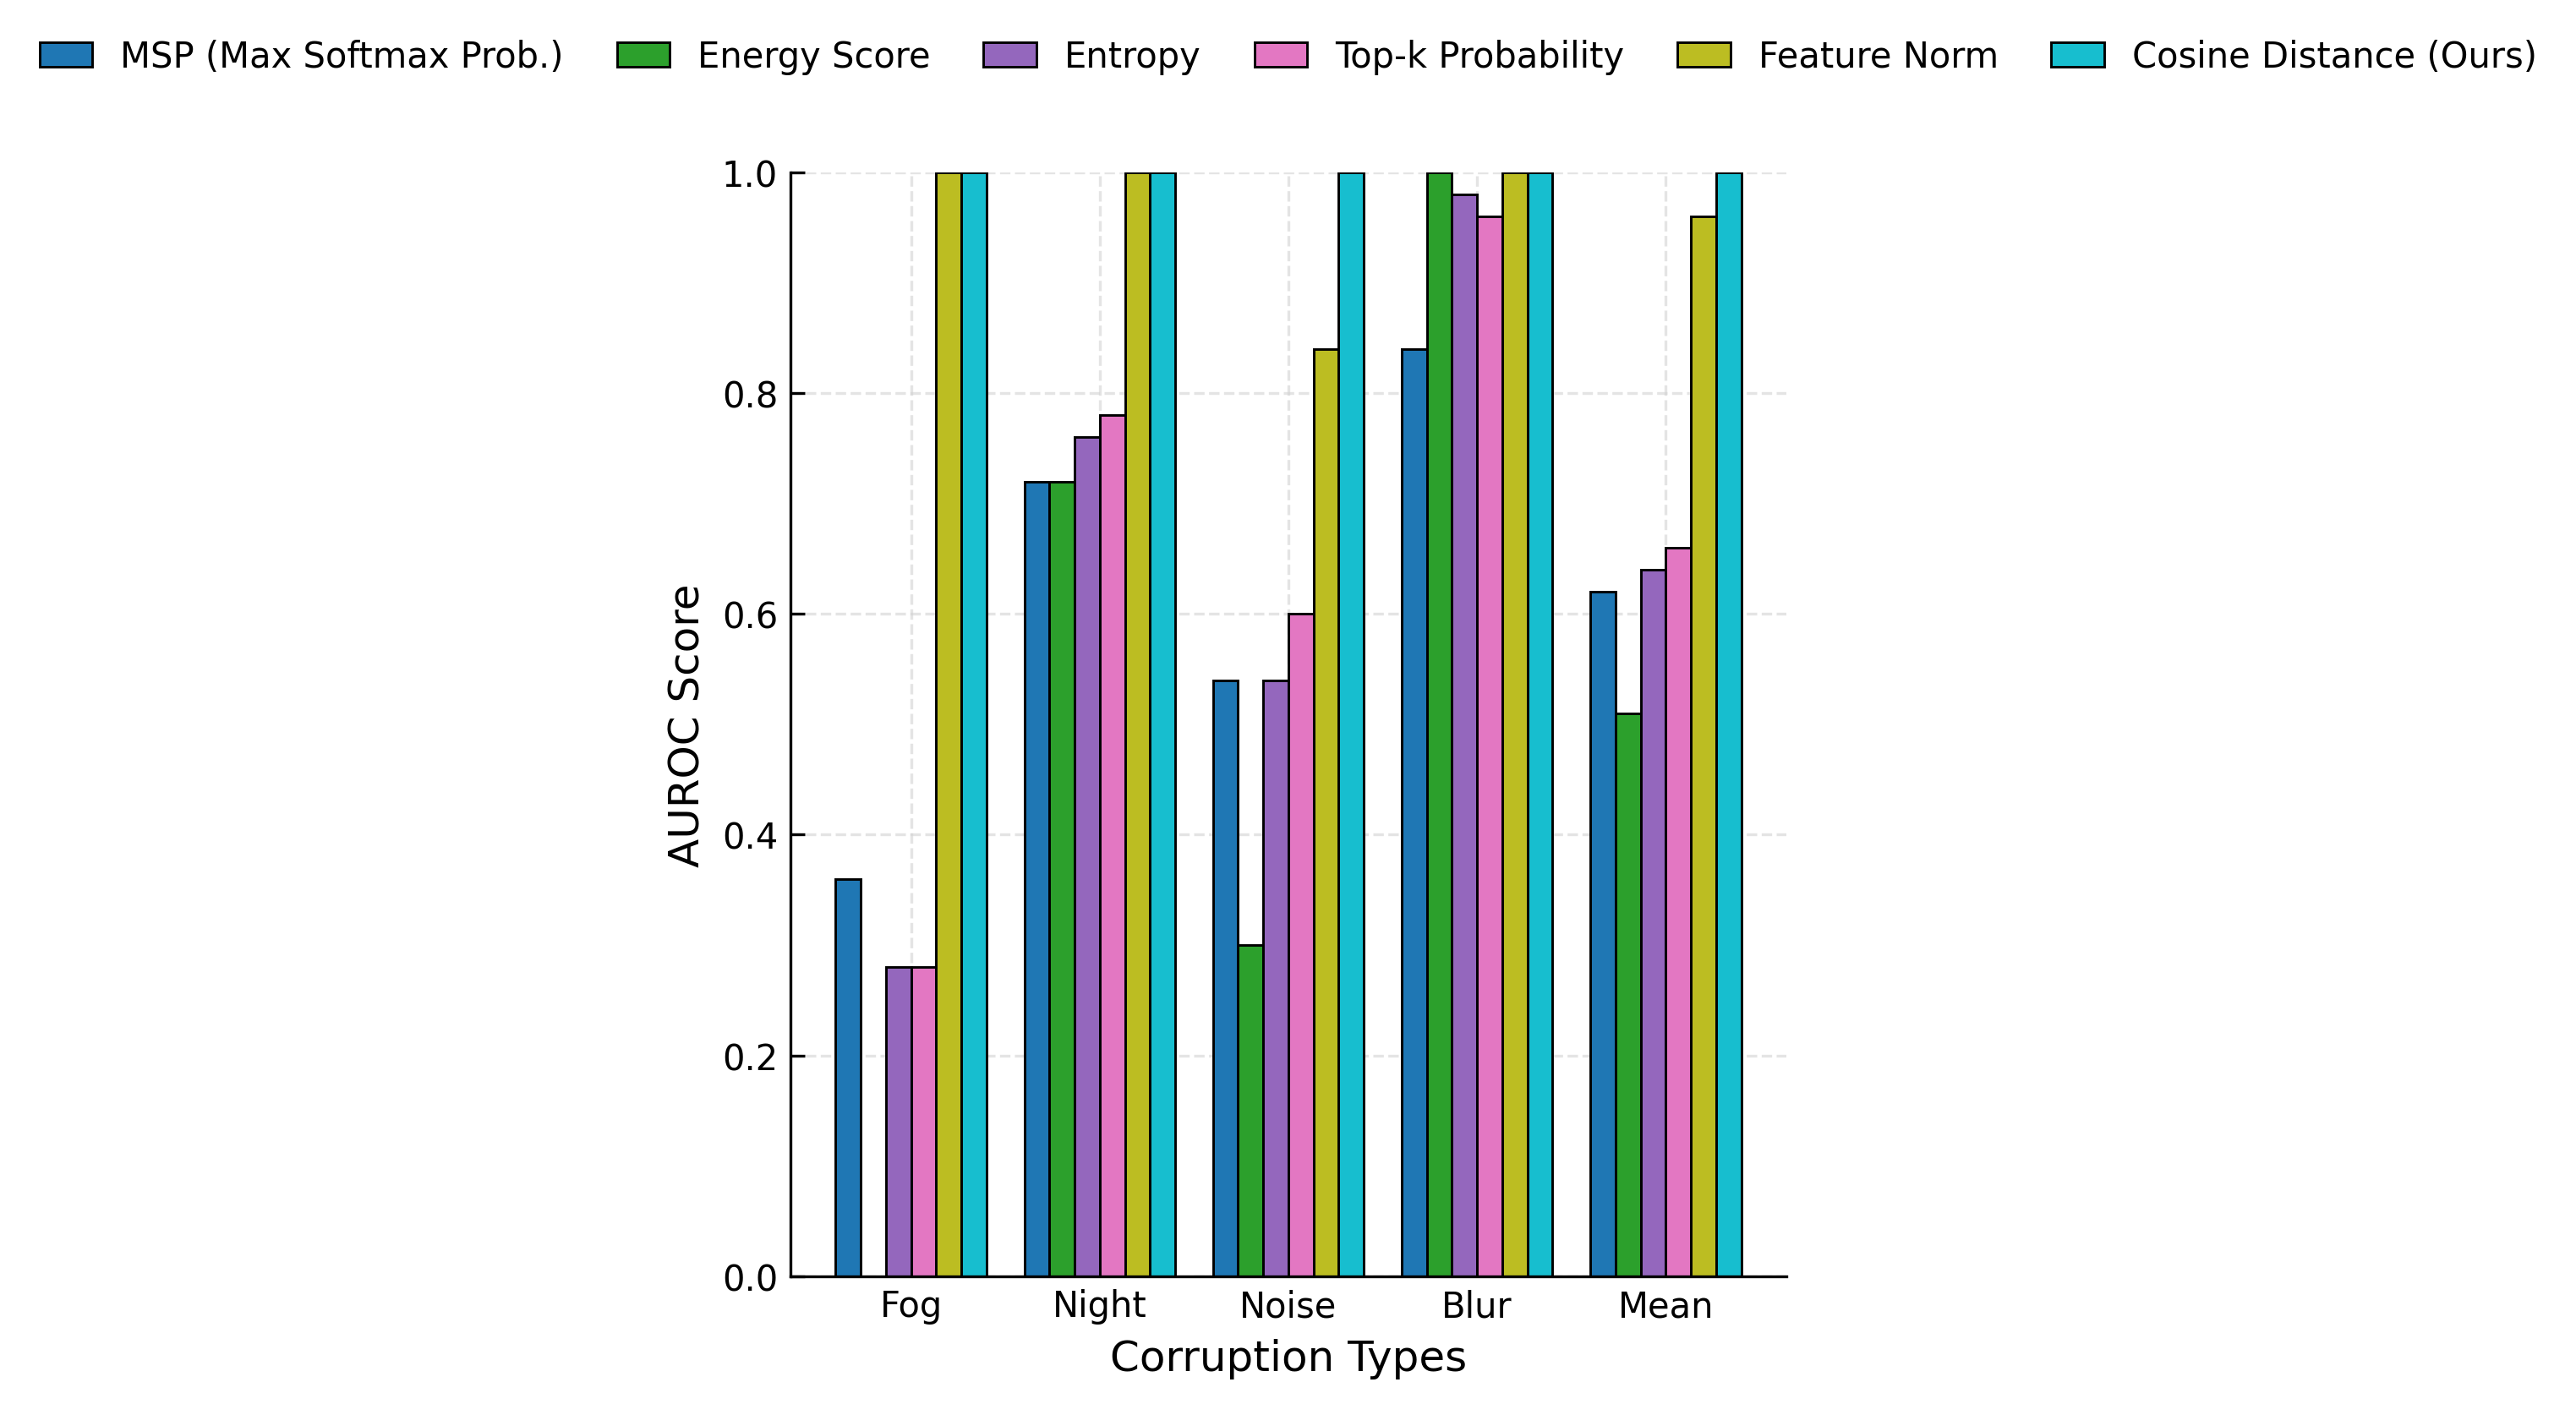
\includegraphics[width=0.95\textwidth]{figures_pb/fig2_main_results.png}
\caption{OOD detection AUROC across methods and corruption types. Output-based methods (MSP, energy, entropy) fail on fog and noise. Feature norm is a strong baseline but degrades on noise (0.84). Cosine distance achieves AUROC\,$=$\,1.0 across all corruptions.}
\label{fig:main_results}
\end{figure}

Energy score is worst, \emph{inverting} the ranking for fog (AUROC\,$=$\,0.0).
Feature norm is the strongest baseline (mean 0.96) but fails on noise (0.84).
The failure of output-based methods reflects our confidence analysis: the model cannot distinguish clean from corrupted at the output level.

\textbf{Statistical certification.}
Bootstrap analysis (1000 resamples) confirms AUROC\,$=$\,1.0 with 95\% CI $[1.0, 1.0]$ for all four corruptions.
Cohen's $d$ ranges from 3.64 (noise, hardest) to 78.62 (night, easiest), with zero overlap between clean and corrupted distance distributions.

\subsection{Calibration Efficiency and Cross-Scene Transfer}
\label{sec:transfer}

\textbf{Minimal calibration.}
Table~\ref{tab:calibration_size} shows AUROC as a function of calibration set size.
Fog, night, and blur achieve perfect detection with $n = 1$.
Noise reaches 0.96 with $n = 1$ and converges to 1.0 at $n = 20$.

\begin{table}[t]
\centering
\caption{AUROC vs.\ number of calibration images. Three of four corruptions are perfectly detected with a single image.}
\label{tab:calibration_size}
\small
\begin{tabular}{lcccc}
\toprule
$n$ & \textbf{Fog} & \textbf{Night} & \textbf{Noise} & \textbf{Blur} \\
\midrule
1 & 1.00 & 1.00 & 0.96 $\pm$ 0.06 & 1.00 \\
2 & 1.00 & 1.00 & 0.98 $\pm$ 0.02 & 1.00 \\
5 & 1.00 & 1.00 & 0.99 $\pm$ 0.02 & 1.00 \\
10 & 1.00 & 1.00 & 0.99 $\pm$ 0.02 & 1.00 \\
20 & 1.00 & 1.00 & 1.00 $\pm$ 0.00 & 1.00 \\
\bottomrule
\end{tabular}
\end{table}

\begin{figure}[t]
\centering
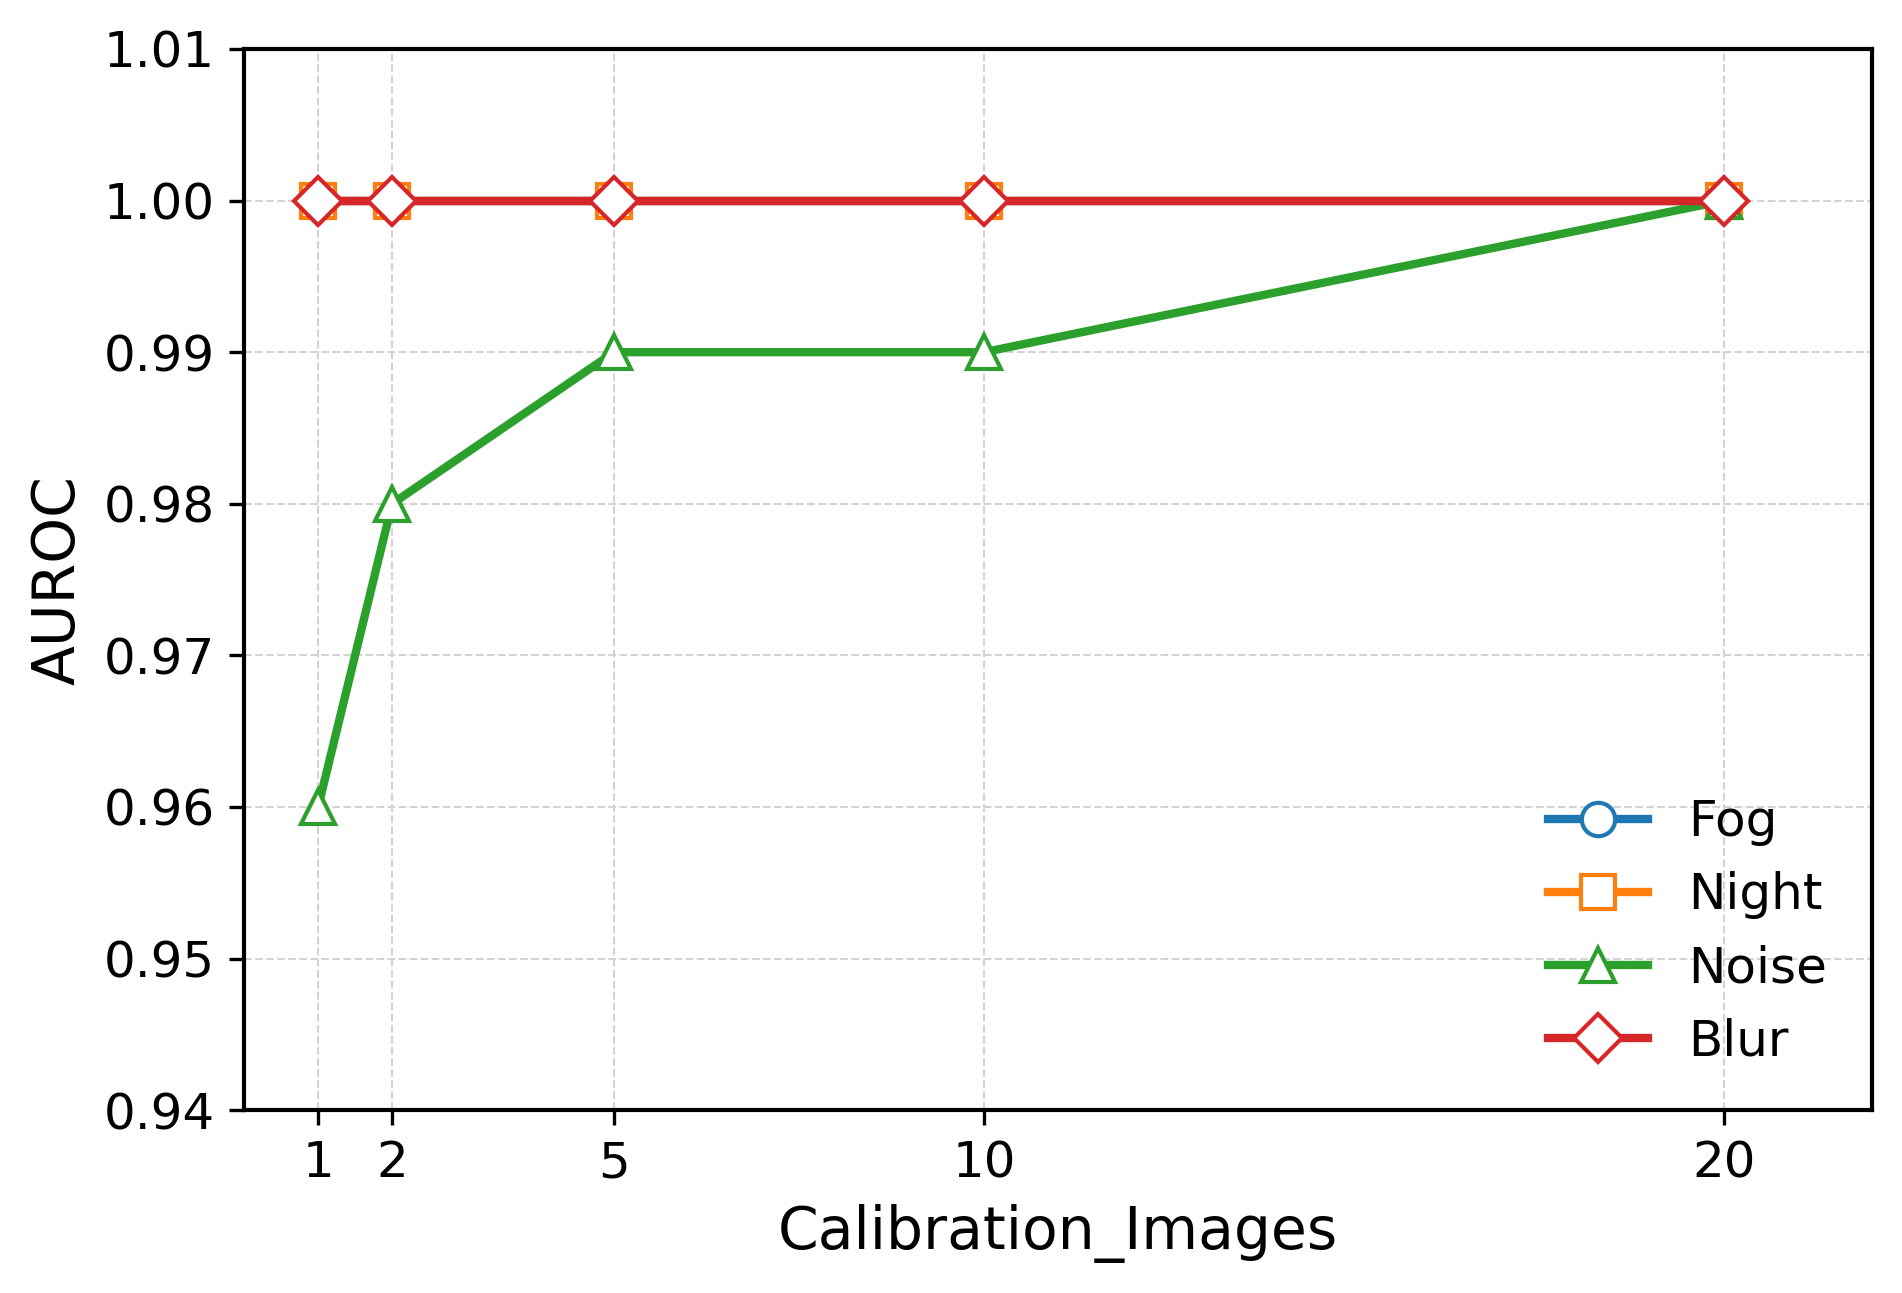
\includegraphics[width=0.95\textwidth]{figures_pb/fig3_calibration.png}
\caption{Calibration efficiency: AUROC converges rapidly with calibration set size. Fog, night, and blur achieve 1.0 with $n = 1$; noise converges at $n = 20$.}
\label{fig:calibration}
\end{figure}

\textbf{Cross-scene transfer.}
Three disjoint scene sets (5 scenes each): all 9 cross-set combinations achieve AUROC\,$=$\,1.0.
Leave-one-out CV across 15 scenes: every held-out scene achieves AUROC\,$=$\,1.0.
Centroid similarity between scene sets exceeds 0.99998.
This establishes: \emph{calibrate once on any scenes, deploy anywhere}.

\textbf{Prompt invariance.}
8 action prompts (13--65 characters) all achieve AUROC\,$=$\,1.0, with cross-prompt similarity $> 0.994$.

\subsection{Severity as a Continuous Signal}
\label{sec:severity}

Cosine distance encodes corruption severity monotonically (Table~\ref{tab:severity}).
The detector identifies embedding shifts \emph{before} actions change: fog distance departs from zero at severity 0.05, but the predicted action token does not change until severity 0.6.

\begin{table}[t]
\centering
\caption{Cosine distance scales monotonically with severity ($R^2 = 0.83\text{--}0.99$). ``Action Change'' is the minimum severity where the predicted action token differs from clean.}
\label{tab:severity}
\small
\begin{tabular}{lcccccc}
\toprule
\textbf{Corruption} & \textbf{Sev 0.1} & \textbf{Sev 0.25} & \textbf{Sev 0.5} & \textbf{Sev 1.0} & $R^2$ & \textbf{Action $\Delta$} \\
\midrule
Fog & $2.0{\times}10^{-5}$ & $3.2{\times}10^{-5}$ & $6.9{\times}10^{-5}$ & $4.3{\times}10^{-4}$ & 0.83 & 0.6 \\
Night & $7.5{\times}10^{-5}$ & $4.2{\times}10^{-4}$ & $1.6{\times}10^{-3}$ & $6.4{\times}10^{-3}$ & 0.93 & 0.3 \\
Noise & $1.8{\times}10^{-5}$ & $3.4{\times}10^{-5}$ & $7.8{\times}10^{-5}$ & $2.0{\times}10^{-4}$ & 0.91 & 0.35 \\
Blur & $1.3{\times}10^{-4}$ & $9.5{\times}10^{-4}$ & $2.6{\times}10^{-3}$ & $4.5{\times}10^{-3}$ & 0.99 & 0.1 \\
\bottomrule
\end{tabular}
\end{table}

\begin{figure}[t]
\centering
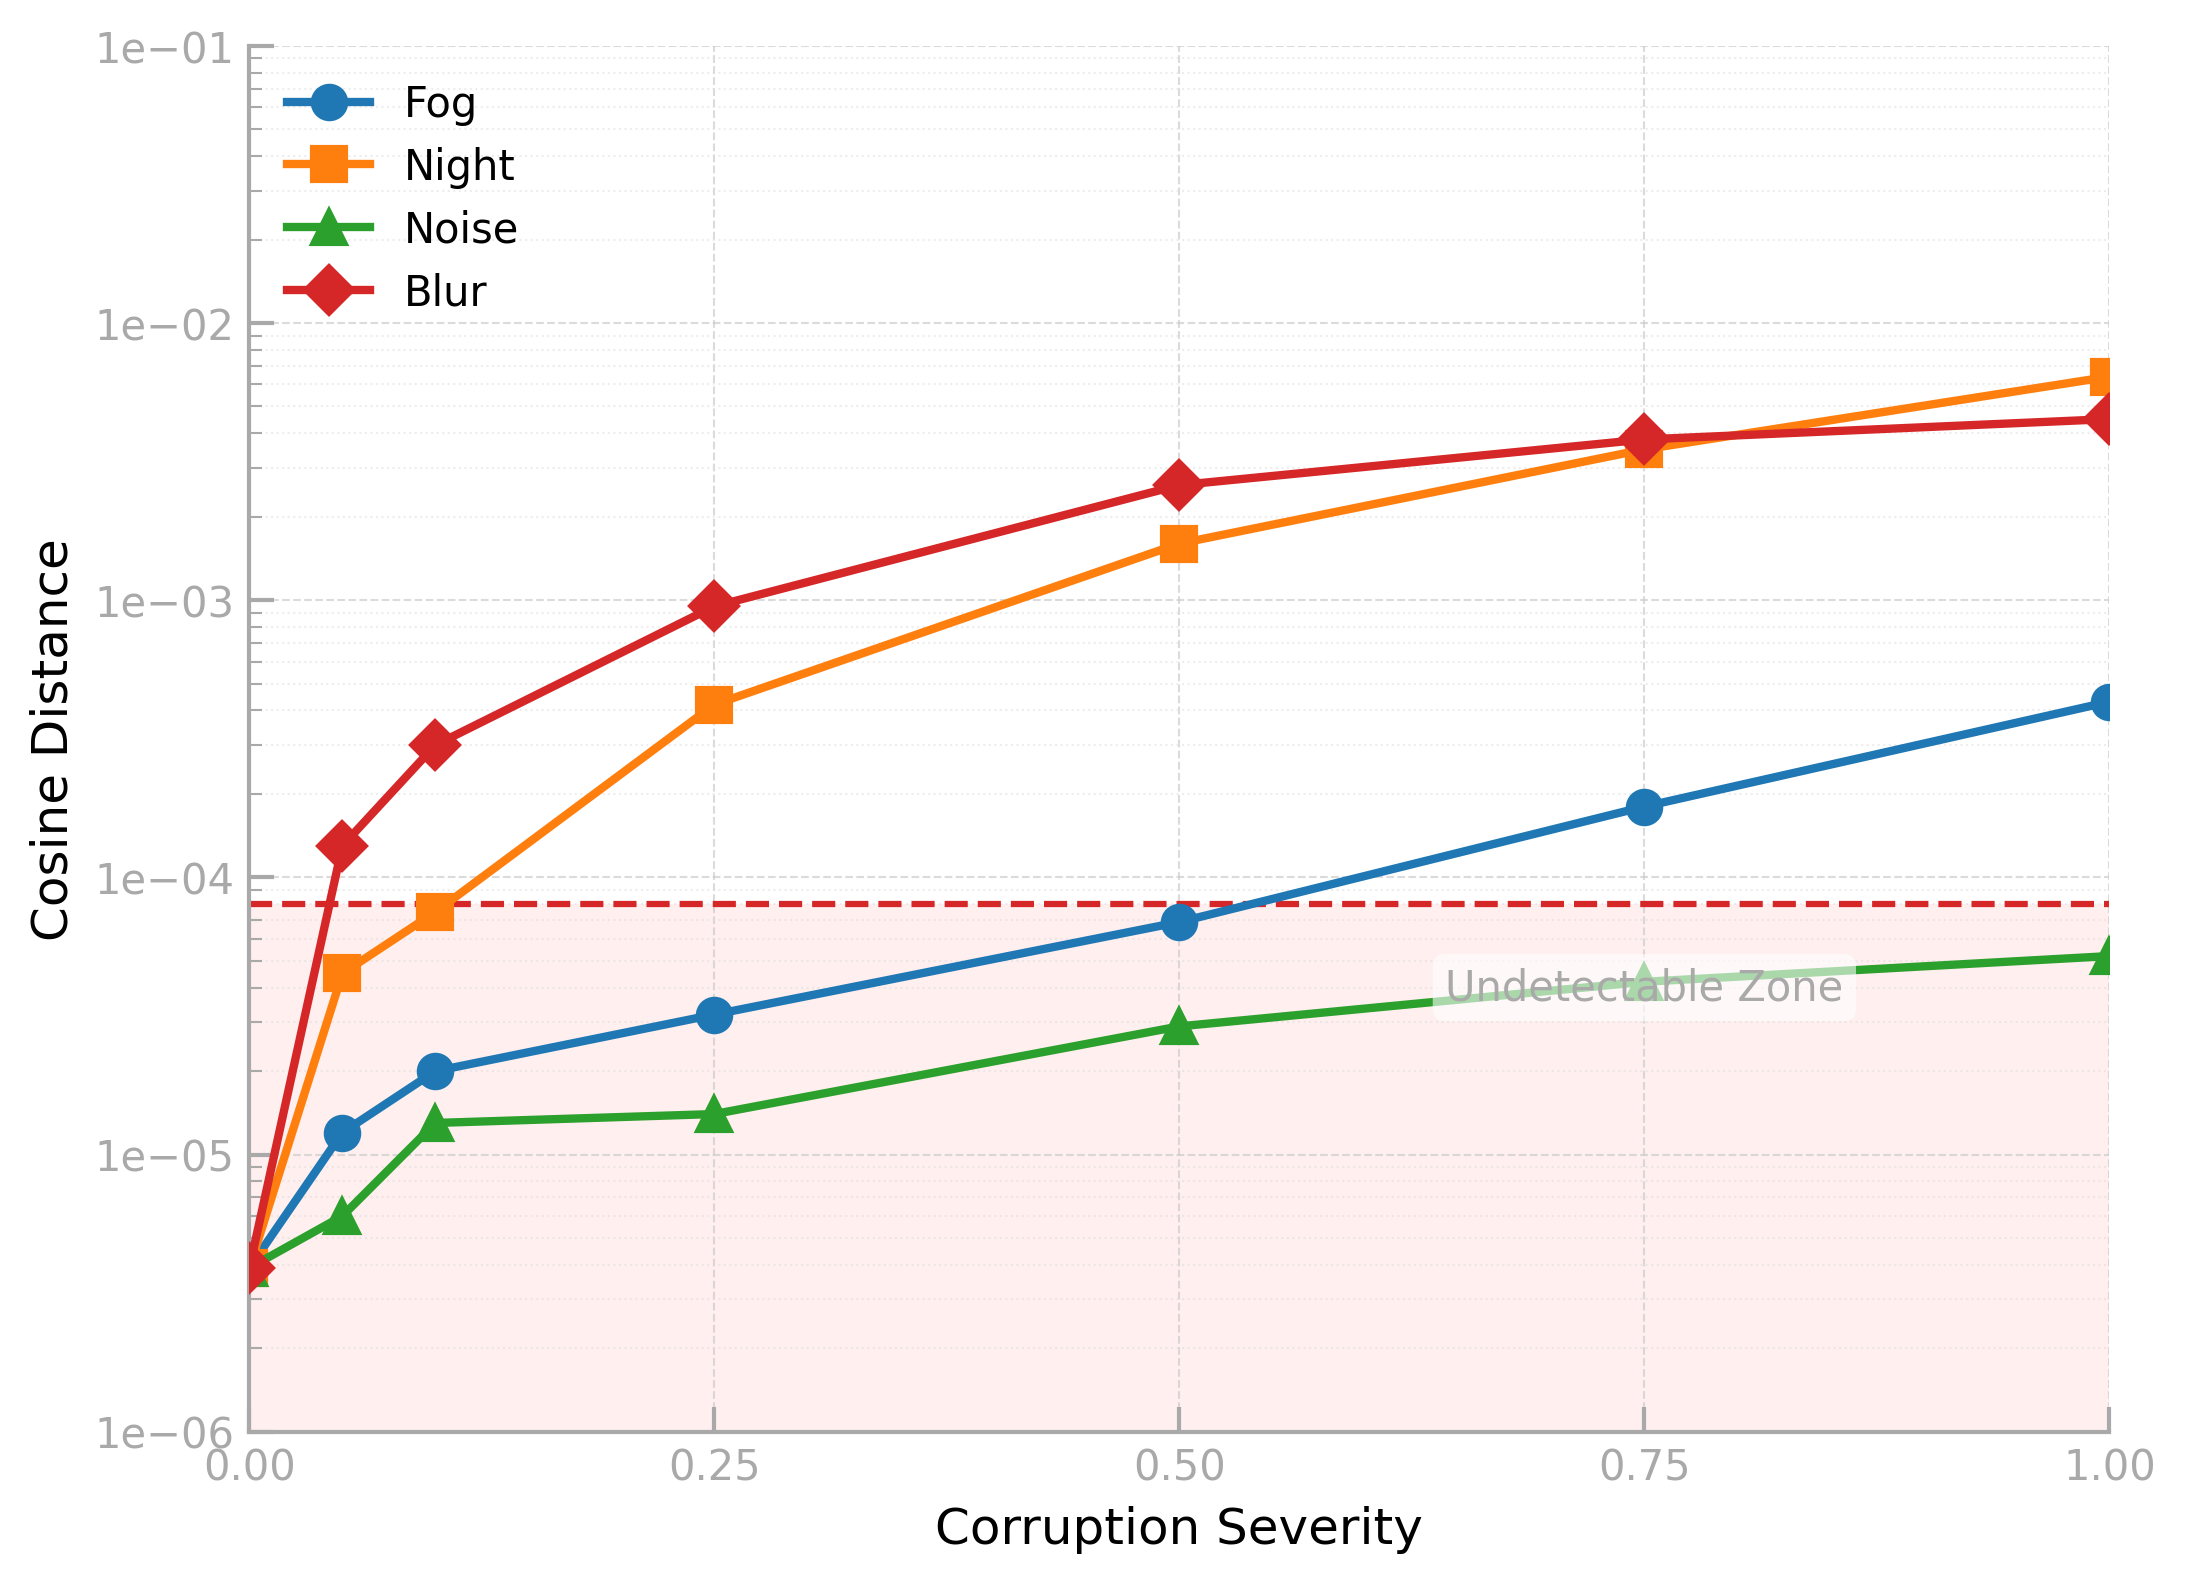
\includegraphics[width=0.95\textwidth]{figures_pb/fig4_severity.png}
\caption{Cosine distance vs.\ corruption severity (log scale). Shaded region: below $3\sigma$ threshold (undetectable). Blur and night cross the threshold at severity $\leq 0.1$; noise crosses near severity $0.5$.}
\label{fig:severity}
\end{figure}

\textbf{Corruption classification.}
The same embedding supports 4-way type classification with 100\% accuracy at full severity and 96.9\% at severity 0.25, enabling a complete pipeline: detect $\to$ classify $\to$ estimate severity $\to$ respond.

\subsection{Computational Overhead}
\label{sec:overhead}

\begin{table}[t]
\centering
\caption{Computational overhead on NVIDIA A40. The detection pipeline adds 14.6\,$\mu$s---three orders of magnitude below the forward pass.}
\label{tab:overhead}
\small
\begin{tabular}{lrl}
\toprule
\textbf{Operation} & \textbf{Time} & \textbf{Notes} \\
\midrule
Forward pass (baseline) & 123.4\,ms & Without hidden states \\
Forward pass (with hidden states) & 129.4\,ms & +5.95\,ms (+4.8\%) \\
Hidden state extraction & 6.7\,$\mu$s & Layer 3, last token \\
Cosine distance & 7.6\,$\mu$s & $d = 4096$ \\
Threshold comparison & 0.3\,$\mu$s & Single float \\
\midrule
\textbf{Post-forward overhead} & \textbf{14.6\,$\mu$s} & \textbf{0.01\% of forward pass} \\
\bottomrule
\end{tabular}
\end{table}

The 5.95\,ms forward-pass increase is PyTorch bookkeeping (tensor storage), not computation; it can be eliminated by modifying the forward method to return only the needed layer.

\subsection{Layer Sweep}
\label{sec:layer_sweep}

\begin{figure}[t]
\centering
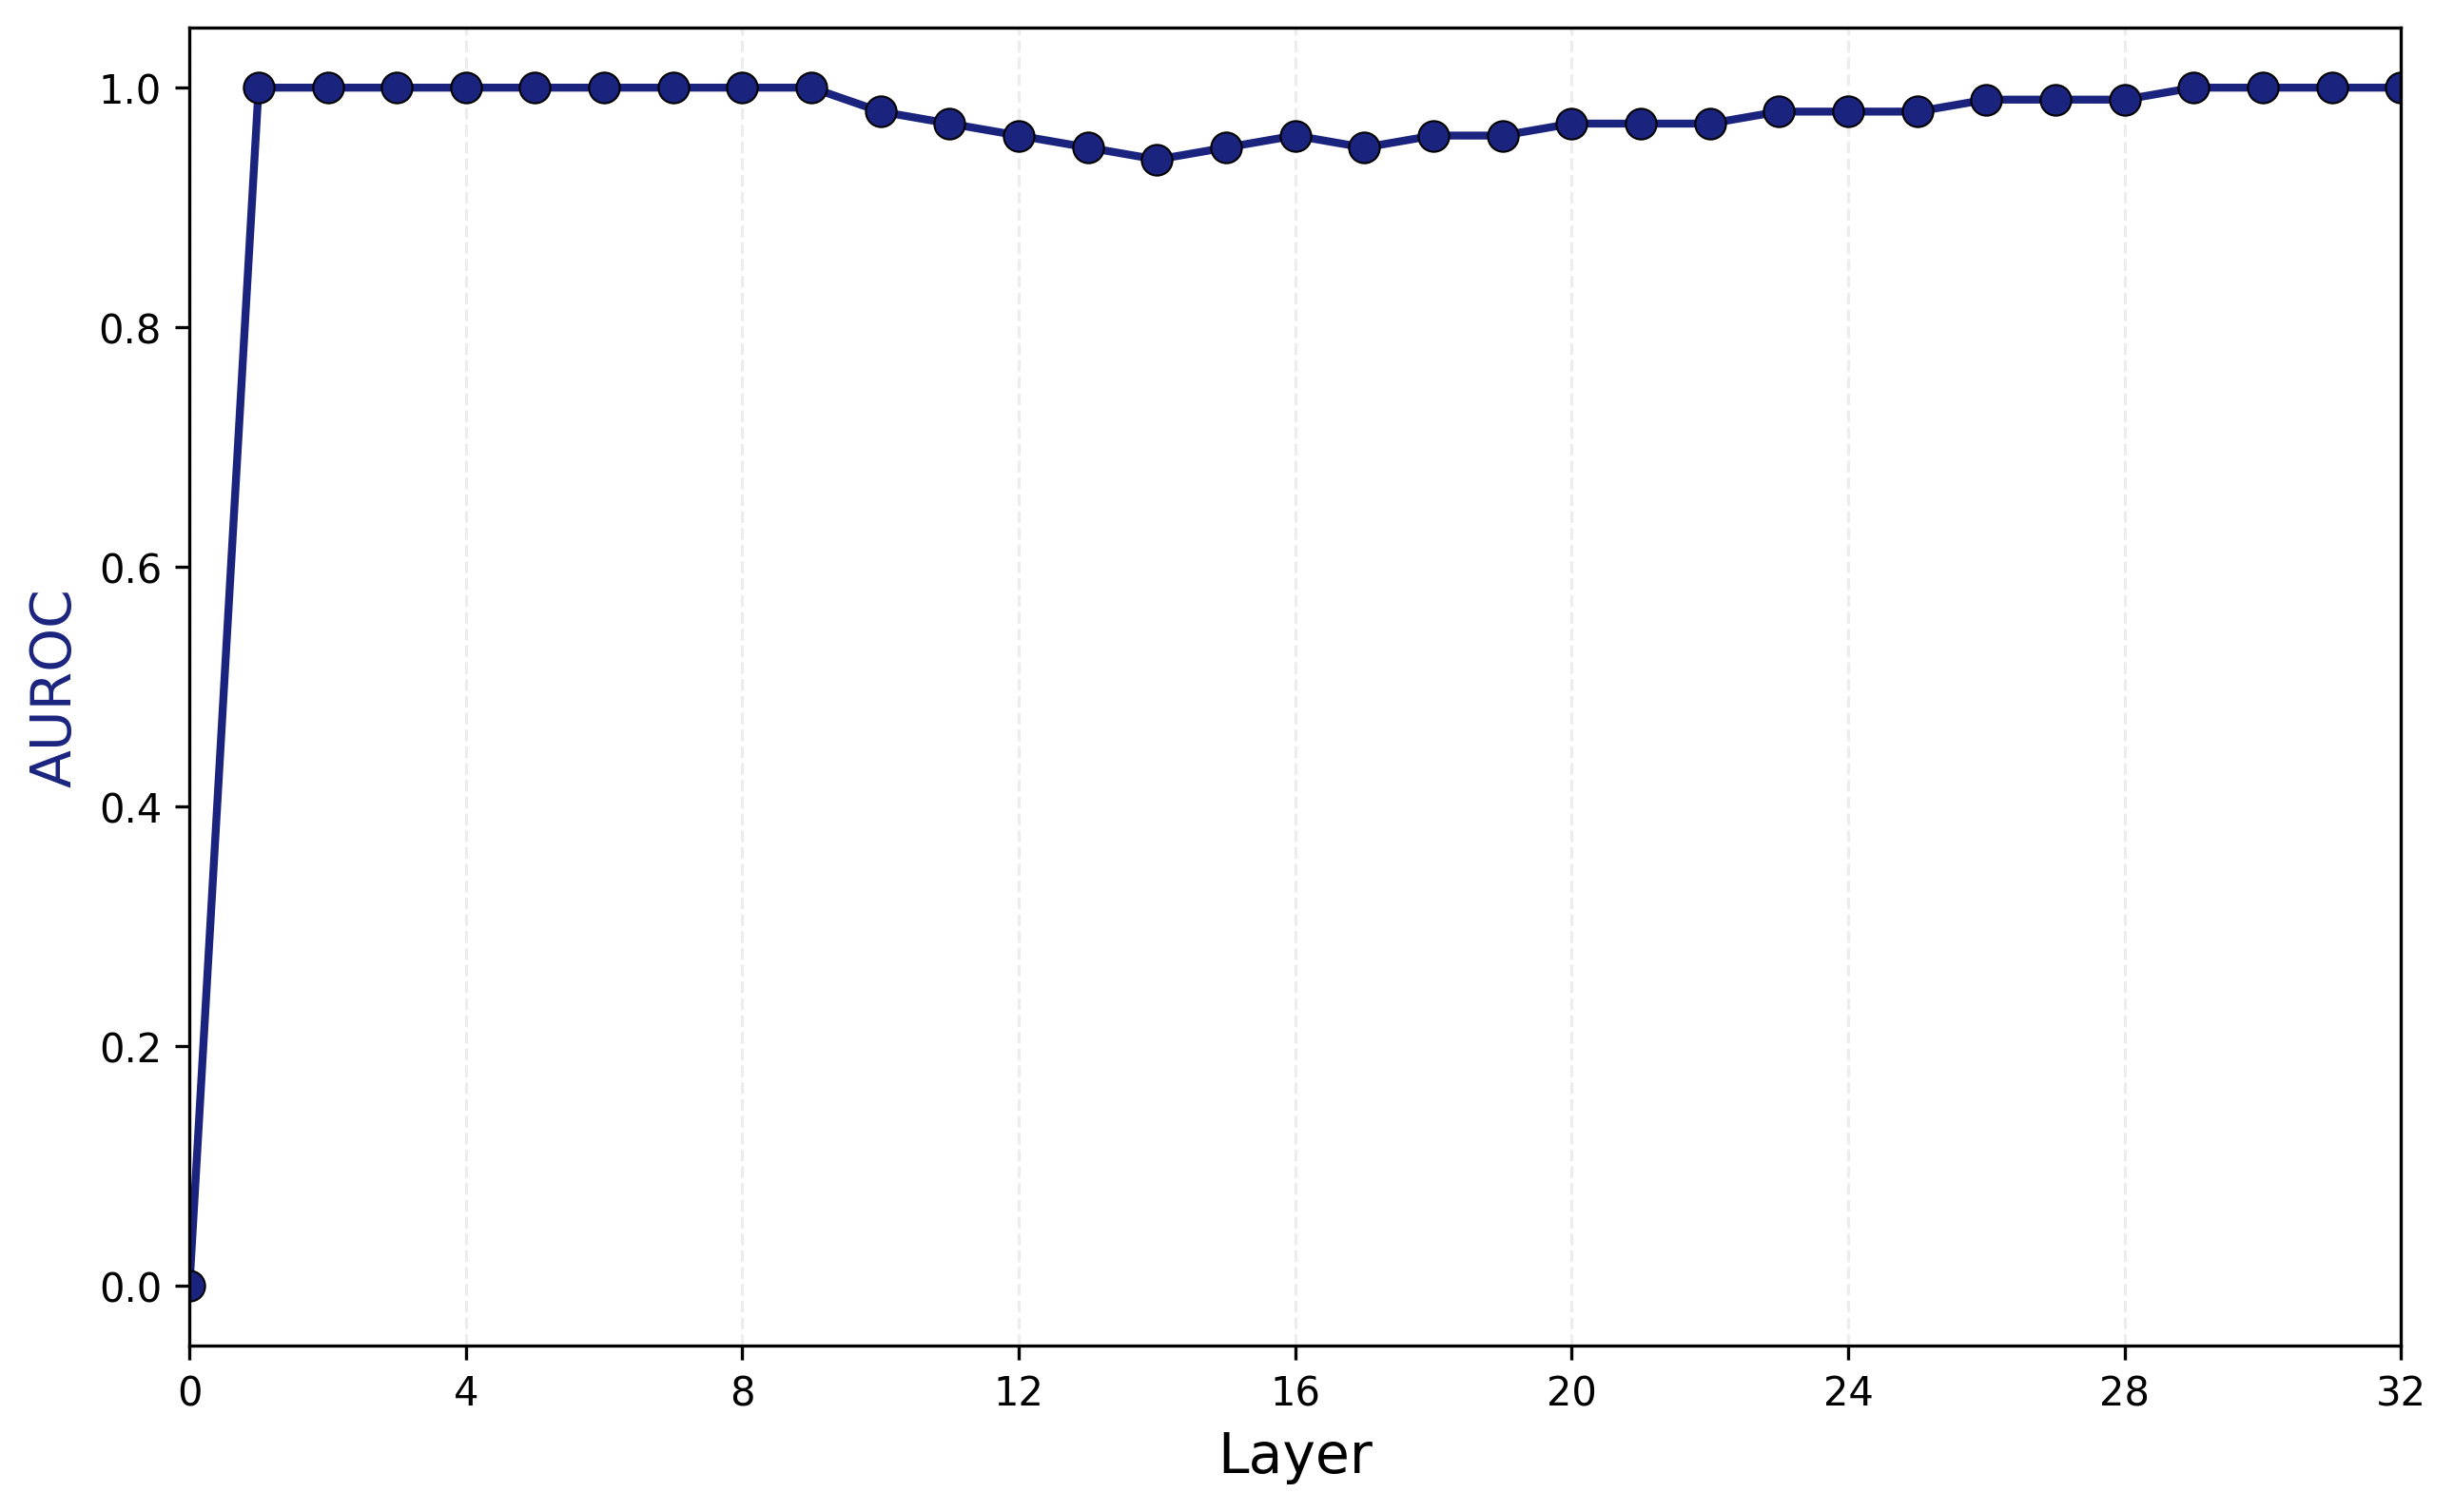
\includegraphics[width=0.95\textwidth]{figures_pb/fig5_layer_sweep.png}
\caption{Per-layer OOD detection AUROC across all 33 layers of OpenVLA-7B. Layer 0 (raw embedding) has zero detection power. Layers 1--9 achieve AUROC\,$=$\,1.0 with layer 1 providing the best separation ratio (256.9$\times$). Middle layers (10--20) show a mild dip driven by noise. Late layers (29--32) recover to 1.0.}
\label{fig:layer_sweep}
\end{figure}

Key findings from the sweep (Figure~\ref{fig:layer_sweep}):
\textbf{Layer 0 is blind} (AUROC\,$=$\,0.0): the raw embedding before transformer processing contains no OOD signal.
\textbf{Layer 1 is optimal}: AUROC\,$=$\,1.0 with separation ratio 256.9$\times$; detection power emerges immediately after the first transformer block.
\textbf{Layers 1--9 and 30--32 are all perfect} (AUROC\,$=$\,1.0).
\textbf{Middle layers show a mild dip}: layer 14 is worst at AUROC\,$=$\,0.9375, driven entirely by noise.
At low severity (0.1), early layers are best: layer 5 achieves AUROC\,$=$\,0.898 vs.\ 0.684 at layer 17.

%==============================================================================
\section{Mechanistic Analysis}
\label{sec:mechanism}
%==============================================================================

\subsection{Why Perfect Detection: Determinism and the Noise Floor}

The method's effectiveness rests on model determinism.
We verify that 5 repeated forward passes produce \textbf{bit-identical} embeddings (max absolute difference $= 0.0$, cosine distance $= 0.0$).
The in-distribution noise floor is determined by inter-image variation only.

Across 30 clean scenes (435 pairwise distances): mean $= 1.07 \times 10^{-4}$, std $= 3.39 \times 10^{-5}$.
Signal-to-noise ratios (corruption distance / noise floor std):
\begin{itemize}
    \item Blur at severity 0.05: SNR $= 17.0$ (reliable)
    \item Night at severity 0.10: SNR $= 4.8$
    \item Fog at severity 0.15: SNR $= 6.0$
    \item Noise at severity 0.50: SNR $= 2.3$ (hardest corruption)
\end{itemize}

Minimum detectable severity ($3\sigma$ crossing): blur at 0.03, night at 0.09, fog at 0.11, noise at 0.45.
Noise is the hardest corruption, requiring moderate severity for reliable detection.

\subsection{The Signal Is in Hidden States, Not Attention}

We measure attention pattern similarity between clean and corrupted inputs:
\begin{itemize}
    \item \textbf{Layer 3 (detection layer)}: cosine similarity 0.9998--0.9999 across all corruptions. The model attends to the same tokens identically.
    \item \textbf{Layer 31 (deep layer)}: similarity drops to 0.82 for night/blur, 0.94--0.95 for fog/noise. Corruption effects on attention grow through depth.
\end{itemize}

The causal mechanism: corrupted visual tokens carry different \emph{values} from the vision encoder $\to$ propagate through \emph{stable} attention routing $\to$ shift the hidden state geometrically $\to$ cosine distance detects the shift.
An attention-based detector would fail at layer 3 where hidden-state monitoring succeeds.

\subsection{Feature Attribution}

The top-50 most discriminative dimensions are largely corruption-specific: only 3 dimensions (of 4096) appear in all four types' top-50 lists.
Despite this, the signal is broadly distributed:
10 random dimensions achieve AUROC $= 0.991$; 500 random dimensions achieve AUROC $= 1.0$.
The detector is robust to dimension selection.

\subsection{Information-Theoretic Analysis}

Mutual information between the embedding and corruption class (5-way) is 2.32 bits---the theoretical maximum ($\log_2 5$), confirming sufficient information for perfect classification.
Rate-distortion analysis: 1-bit quantization per dimension suffices for AUROC $\geq 0.95$.
Channel capacity reaches 1.0 bit at severity $\geq 1.0$ for all corruptions.

%==============================================================================
\section{Dual Failure Modes in VLA Actions}
\label{sec:failure_modes}
%==============================================================================

We identify two qualitatively distinct behavioral failure modes:

\textbf{Fog: Overconfident action collapse.}
Under fog, the model produces only 1.4 unique tokens per dimension (vs.\ 6.7 clean), converging to nearly identical \emph{wrong} actions.
Confidence \emph{increases}---the model commits to the wrong action with high certainty.
This is the most dangerous mode: a confident wrong action executed without hesitation.

\textbf{Night: Uncertainty explosion.}
Night corruption doubles action entropy from 1.66 to 3.42 nats/token.
The model spreads probability across many tokens, \emph{decreasing} confidence.
This failure is partially self-diagnosing.

The hidden-state detector flags both (AUROC\,$=$\,1.0), but a complete safety system should distinguish them---overconfident collapse requires immediate intervention, while uncertainty explosion may allow graceful degradation.

%==============================================================================
\section{Limitations and Failure Modes}
\label{sec:limitations}
%==============================================================================

\begin{figure}[t]
\centering
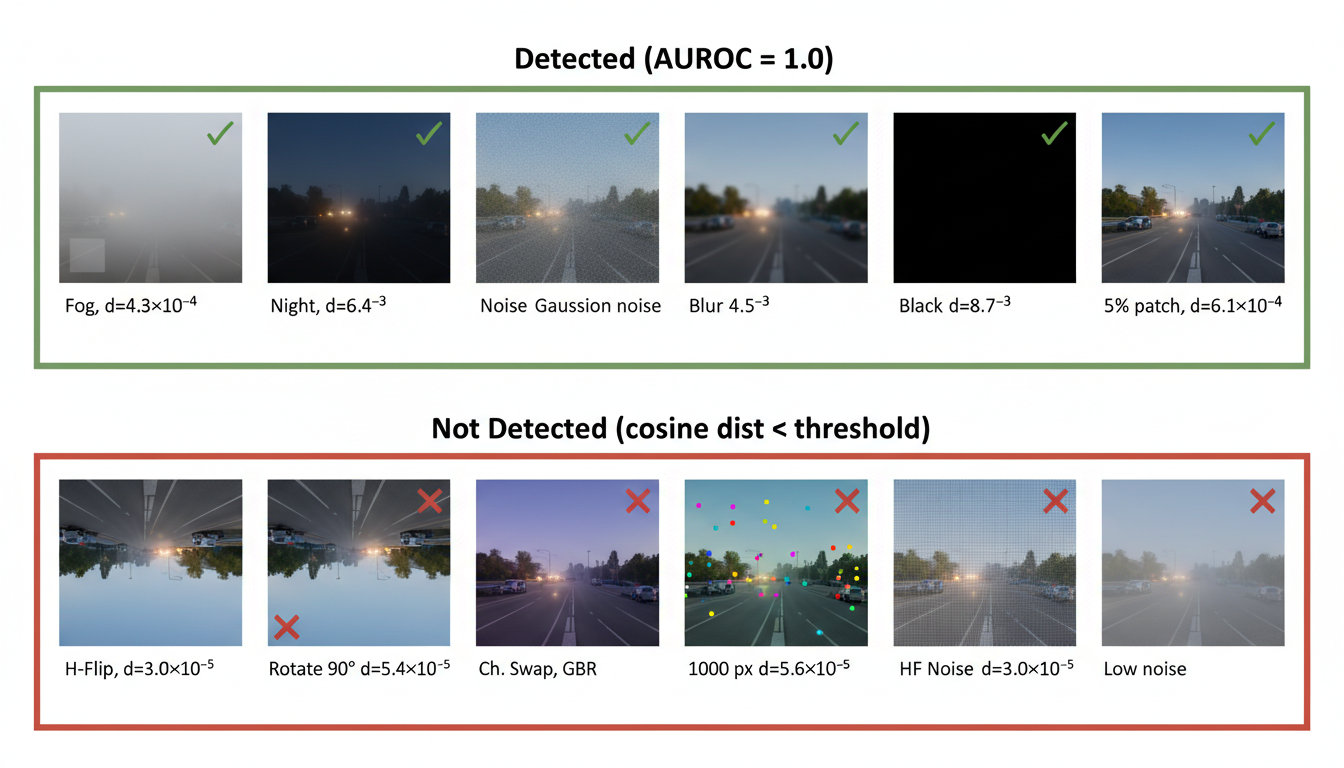
\includegraphics[width=0.98\textwidth]{figures_pb/fig_failure_modes.png}
\caption{\textbf{What the detector can and cannot detect.} \emph{Top (green)}: Distributional corruptions---fog, night, noise, blur, black images, and even a 5\% pixel patch---are reliably detected. \emph{Bottom (red)}: Geometric transformations (flips, rotations), channel swaps, sparse pixel edits, and low-severity noise remain invisible. The detector captures distributional corruption, not geometric perturbation.}
\label{fig:failure_modes}
\end{figure}

We systematically characterize what the method \emph{cannot} detect (Figure~\ref{fig:failure_modes}).

\textbf{Geometric perturbations are invisible.}
None of the following are flagged: pixel changes (1--1000 pixels), channel swaps (GBR, BRG), horizontal flips, 90-degree rotations.
This is fundamental: the detector captures distributional corruption, not geometric transformation.

\textbf{Low-severity noise evades detection.}
Gaussian noise below severity 0.45 has SNR $< 3$.
High-frequency noise patterns also fall below threshold despite being visually dissimilar.

\textbf{Corruption order matters.}
Blur-then-noise can produce a false negative ($4.45 \times 10^{-5}$, below threshold), while noise-then-blur is detected normally ($6.71 \times 10^{-3}$).

\textbf{Single model evaluation.}
All results are from OpenVLA-7B.
The mechanistic arguments (determinism, stable attention, distributed signal) should generalize to other VLAs in eval mode, but empirical validation on additional architectures (RT-2, $\pi_0$) remains future work.

\textbf{Partial corruption.}
On the positive side, a $50\times50$ pixel patch ($\sim$5\% of $224\times224$) produces cosine distance $6.1 \times 10^{-4}$---$7.6\times$ above threshold, reliably detected.

\textbf{Adversarial attacks.}
Gradient-based attacks (PGD, FGSM) are not evaluated and represent an important direction for future work.

%==============================================================================
\section{Discussion}
\label{sec:discussion}
%==============================================================================

\textbf{Why are the results so clean?}
AUROC\,$=$\,1.0 follows from two properties: (1) model determinism sets in-distribution variance to zero, and (2) visual corruptions induce non-trivial embedding shifts.
With a noise floor of $\sim$$10^{-4}$ and corruption signals of $10^{-3}\text{--}10^{-2}$, perfect separation is the \emph{expected} outcome.
The more informative results are the severity gradients (when does detection degrade?) and failure modes (what escapes detection?).

\textbf{Compound corruptions.}
All pairwise, triple, and quadruple compound scenarios achieve AUROC\,$=$\,1.0.
Distances are sub-additive: the dominant corruption determines the embedding direction while the weaker modulates magnitude.
Fog\,$+$\,noise produces the lowest compound distance ($1.56 \times 10^{-3}$) due to anti-correlated shifts (cosine similarity $-0.53$).

\textbf{Temporal deployment.}
In frame-by-frame simulation (50 trials $\times$ 100 frames), the detector achieves zero false alarms on clean streams and flags corruption on the first corrupted frame.

\textbf{Online adaptation.}
The centroid can be updated via exponential moving average ($\alpha = 0.01\text{--}0.1$), converging within $\sim$10 frames while maintaining AUROC\,$=$\,1.0 under gradual distribution shift.

\textbf{Broader implications.}
The gap between uninformative output confidence and perfectly informative hidden states suggests that VLA safety monitoring should look \emph{inside} the model, not at its outputs.
This principle---\emph{hidden states know what confidence doesn't}---may extend to other deployed AI systems.

%==============================================================================
\section{Conclusion}
\label{sec:conclusion}
%==============================================================================

We have shown that cosine distance of hidden-state embeddings from a clean centroid provides perfect OOD detection for OpenVLA-7B across four visual corruption types.
The method requires 2 calibration images, adds 14.6\,$\mu$s overhead, and transfers across scenes without recalibration.
We provide a mechanistic account rooted in model determinism and stable attention, and comprehensively characterize failure modes.
Future work should validate across VLA architectures, evaluate adversarial robustness, and explore semantic OOD detection (novel objects, unusual scenes) beyond distributional corruptions.

%==============================================================================
\section*{Broader Impact Statement}
%==============================================================================

This work develops safety monitoring for VLA models used in robotic control and autonomous driving.
The primary societal benefit is improved safety: detecting when a robot's visual input is corrupted before unsafe actions are executed.
Potential risks include overreliance on the detector (it does not catch geometric perturbations or adversarial attacks) and the possibility that adversaries could craft inputs that evade detection while causing harmful actions.
We mitigate this by thoroughly documenting failure modes.
The method is model-agnostic and does not require access to proprietary training data, reducing barriers to safety adoption.

%==============================================================================
\section*{Reproducibility Statement}
%==============================================================================

All experiments use the publicly available OpenVLA-7B model~\cite{kim2024openvla} on a single NVIDIA A40 GPU.
Visual corruptions are defined by closed-form transformations (specified in \S\ref{sec:experiments}).
The detection method (Algorithm~\ref{alg:detection}) requires no training, only a centroid from $\geq$2 clean images.
Complete code, experiment scripts, all raw JSON results, and generated figures are available at \url{https://github.com/sreedath/Vizuara-VLA-Research}.

%==============================================================================
\begin{thebibliography}{30}

\bibitem{kim2024openvla}
M.~J. Kim, K.~Pertsch, S.~Karamcheti, T.~Xiao, A.~Balakrishna, S.~Nair, R.~Rafailov, E.~Foster, G.~Lam, P.~Sanketi, Q.~Vuong, T.~Kollar, B.~Burchfiel, R.~Tedrake, D.~Sadigh, S.~Levine, P.~Liang, and C.~Finn.
\newblock {OpenVLA}: An open-source vision-language-action model.
\newblock In \emph{CoRL}, 2024.

\bibitem{brohan2023rt2}
A.~Brohan, N.~Brown, J.~Carbajal, Y.~Chebotar, X.~Chen, K.~Choromanski, T.~Ding, D.~Driess, A.~Dubey, C.~Finn, et~al.
\newblock {RT-2}: Vision-language-action models transfer web knowledge to robotic control.
\newblock In \emph{CoRL}, 2023.

\bibitem{black2024pi0}
K.~Black, N.~Brown, D.~Driess, A.~Esmail, M.~Equi, C.~Finn, N.~Fusai, L.~Groom, K.~Hausman, B.~Ichter, et~al.
\newblock $\pi_0$: A vision-language-action flow model for general robot control.
\newblock \emph{arXiv preprint arXiv:2410.24164}, 2024.

\bibitem{hendrycks2017baseline}
D.~Hendrycks and K.~Gimpel.
\newblock A baseline for detecting misclassified and out-of-distribution examples in neural networks.
\newblock In \emph{ICLR}, 2017.

\bibitem{liang2018enhancing}
S.~Liang, Y.~Li, and R.~Srikant.
\newblock Enhancing the reliability of out-of-distribution image detection in neural networks.
\newblock In \emph{ICLR}, 2018.

\bibitem{liu2020energy}
W.~Liu, X.~Wang, J.~Owens, and Y.~Li.
\newblock Energy-based out-of-distribution detection.
\newblock In \emph{NeurIPS}, 2020.

\bibitem{lee2018mahalanobis}
K.~Lee, K.~Lee, H.~Lee, and J.~Shin.
\newblock A simple unified framework for detecting out-of-distribution samples and adversarial attacks.
\newblock In \emph{NeurIPS}, 2018.

\bibitem{sun2021react}
Y.~Sun, C.~Guo, and Y.~Li.
\newblock {ReAct}: Out-of-distribution detection with rectified activations.
\newblock In \emph{NeurIPS}, 2021.

\bibitem{huang2021importance}
R.~Huang, A.~Geng, and Y.~Li.
\newblock On the importance of gradients for detecting distributional shifts in visual tasks.
\newblock In \emph{NeurIPS}, 2021.

\bibitem{gal2016dropout}
Y.~Gal and Z.~Ghahramani.
\newblock Dropout as a {B}ayesian approximation: Representing model uncertainty in deep learning.
\newblock In \emph{ICML}, 2016.

\bibitem{kadavath2022language}
S.~Kadavath, T.~Conerly, A.~Askell, T.~Henighan, D.~Drain, E.~Perez, S.~Schiefer, Z.~Hatfield-Dodds, N.~DasSarma, E.~Tran-Phung, et~al.
\newblock Language models (mostly) know what they know.
\newblock \emph{arXiv preprint arXiv:2207.05221}, 2022.

\bibitem{tian2023just}
K.~Tian, E.~Mitchell, H.~Yao, C.~D. Manning, and C.~Finn.
\newblock Just ask for calibration: Strategies for eliciting calibrated confidence scores from language models fine-tuned with human feedback.
\newblock In \emph{EMNLP}, 2023.

\bibitem{zollo2025calibration}
M.~Zollo, A.~Skalse, and J.~Foerster.
\newblock On the calibration of vision-language-action models.
\newblock \emph{arXiv preprint}, 2025.

\bibitem{tian2024drivevlm}
X.~Tian, J.~Gu, B.~Li, Y.~Liu, Y.~Wang, Z.~Zhao, K.~Zhan, P.~Jia, X.~Lang, and H.~Zhao.
\newblock {DriveVLM}: The convergence of autonomous driving and large vision-language models.
\newblock \emph{arXiv preprint arXiv:2402.12289}, 2024.

\bibitem{chen2024autovala}
J.~Chen, Z.~Jiang, D.~Chen, Y.~Liu, Z.~Li, S.~Shan, and X.~Chen.
\newblock {AutoVLA}: Autonomous driving via vision-language-action model.
\newblock \emph{arXiv preprint}, 2024.

\bibitem{sima2025alpamayo}
C.~Sima, Z.~Jiang, W.~Wu, K.~Chen, Y.~Nie, S.~Zhang, X.~Zhou, B.~He, J.~Zhang, Y.~Qiao, et~al.
\newblock {Alpamayo-R1}: Reasoning-augmented driving VLA.
\newblock \emph{arXiv preprint}, 2025.

\bibitem{latentvla2025}
Y.~Wang, Z.~Liu, and Others.
\newblock {LatentVLA}: Latent-space vision-language-action models for efficient robotic control.
\newblock \emph{arXiv preprint}, 2025.

\bibitem{sun2022dice}
Y.~Sun and Y.~Li.
\newblock {DICE}: Leveraging sparsification for out-of-distribution detection.
\newblock In \emph{ECCV}, 2022.

\bibitem{podolskiy2021revisiting}
A.~Podolskiy, D.~Lipin, A.~Bout, E.~Artemova, and I.~Piontkovskaya.
\newblock Revisiting {M}ahalanobis distance for transformer-based out-of-distribution detection.
\newblock In \emph{AAAI}, 2021.

\end{thebibliography}

%==============================================================================
\appendix
\section{Appendix}
%==============================================================================

\subsection{Noise Floor Analysis}
\label{app:noise_floor}

\begin{table}[h]
\centering
\caption{Clean-clean cosine distance distribution (435 pairwise distances from 30 scenes).}
\label{tab:noise_floor}
\small
\begin{tabular}{lr}
\toprule
\textbf{Statistic} & \textbf{Value} \\
\midrule
Mean & $1.066 \times 10^{-4}$ \\
Std & $3.391 \times 10^{-5}$ \\
Min & $4.337 \times 10^{-5}$ \\
Max & $2.352 \times 10^{-4}$ \\
Median & $1.025 \times 10^{-4}$ \\
Within-image variance & 0.0 (deterministic) \\
\bottomrule
\end{tabular}
\end{table}

\subsection{PCA of Corruption Directions}
\label{app:pca}

PCA of the four corruption shift vectors (mean displacement from clean centroid at severity 1.0):
PC1 explains 64.8\% of variance; PC1+PC2: 86.3\%; PC1--PC3: 99.3\%.
PC4 explains only 0.7\%, confirming that four corruption types span an effectively 3D subspace in 4096-D space.

Shift vector norms: night (1.10) $>$ blur (0.94) $>$ fog (0.64) $>$ noise (0.16).
Anti-correlation between fog and noise (cosine similarity $-0.53$) explains sub-additive compound distances.

\subsection{Edge Cases}
\label{app:edge_cases}

\begin{table}[h]
\centering
\caption{Edge case detection results. Threshold $= 8.03 \times 10^{-5}$.}
\label{tab:edge_cases}
\small
\begin{tabular}{lrl}
\toprule
\textbf{Input} & \textbf{Cosine Dist} & \textbf{Detected?} \\
\midrule
All black & $8.71 \times 10^{-3}$ & Yes \\
All white & $6.23 \times 10^{-3}$ & Yes \\
Pure red/green/blue & $4.4\text{--}5.5 \times 10^{-3}$ & Yes \\
Checkerboard & $4.24 \times 10^{-3}$ & Yes \\
HF noise & $2.98 \times 10^{-5}$ & \textbf{No} \\
\midrule
$50\times50$ patch (fog) & $6.07 \times 10^{-4}$ & Yes \\
20px border (fog) & $1.05 \times 10^{-3}$ & Yes \\
Top half (fog) & $1.17 \times 10^{-3}$ & Yes \\
\midrule
1 pixel changed & $5.90 \times 10^{-5}$ & \textbf{No} \\
1000 pixels changed & $5.55 \times 10^{-5}$ & \textbf{No} \\
Channel swap (GBR) & $4.55 \times 10^{-5}$ & \textbf{No} \\
Horizontal flip & $2.96 \times 10^{-5}$ & \textbf{No} \\
Rotate 90$^\circ$ & $5.37 \times 10^{-5}$ & \textbf{No} \\
\bottomrule
\end{tabular}
\end{table}

\subsection{Compound Corruption Results}
\label{app:compound}

All pairwise, triple, and all-four compound corruptions achieve AUROC\,$=$\,1.0.
Compound distances are sub-additive: fog\,$+$\,noise $= 1.56 \times 10^{-3}$ ($<$ fog alone at $3.06 \times 10^{-3}$).
Night\,$+$\,blur produces the highest pairwise distance ($9.67 \times 10^{-3}$).

\subsection{Online Calibration Adaptation}
\label{app:online}

The centroid can be updated online: $\bmu_{t+1} = (1 - \alpha) \bmu_t + \alpha \, \be(\bx_{t+1})$.
With $\alpha = 0.01\text{--}0.1$, EMA centroids converge within $\sim$10 clean frames, maintaining AUROC\,$=$\,1.0 throughout deployment including under gradual distribution shift.
Cold-start with a single calibration image maintains perfect detection for fog, night, and blur; noise achieves AUROC\,$=$\,0.96.

\subsection{Embedding Dynamics Across Depth}
\label{app:dynamics}

Tracking L2 divergence of corruption embeddings from clean through the 33-layer network: divergence is zero at layer 0, detectable at layers 1--9 (where cosine AUROC\,$=$\,1.0), and grows substantially at layers 12--15.
By layer 32: night (0.623) $>$ blur (0.544) $>$ fog (0.256) $>$ noise (0.147).

The amplification factor (corruption divergence / clean variance) peaks at layer 1: night (212$\times$), blur (193$\times$), fog (41$\times$), noise (2.5$\times$).
Silhouette scores peak at layer 2 (0.833) and decrease monotonically.

\end{document}
